% !TeX root = ../documento.tex
\chapter{Fundamentação Teórica}
\label{cap:fundamentacao-teorica}

\section{Freio e sua evolução}
\label{sec:fundamentacao-teorica-a}

Como foi dito, a desenvolvimento cria necessidade, e a evolução na mobilidade humana, saindo de tração animal para veículos automotores, crio a exiguidade de dirigir com segurança, e um dos itens mais importante neste amadurecimento e o freio, mas como é possível amadurecer uma coisa, sem entender seu funcionamento? aqui vai ser abordado alguns modelos de freios e seus funcionamentos.


\subsection{Freios de sapata} 
\label{sec:fundamentacao-teorica-a}

Como vimos, foi adotado pneu e aço nas rodas para a prevenção de desgaste rápido, e o freios de sapata e sapatas externas nas superfícies de rolamento das rodas, foi adotado como forma de desacelerar as carruagens puxadas por cavalos, um primeiro exemplo é a “carruagem” desenvolvida por Gottlieb Daimler como veículo experimental em 1885 Figura~\ref{fig:Motocicleta-Daimler}. Um cabo conduzia da alavanca de acionamento do freio, localizada na parte dianteira, próximo ao braço de direção, até a sapata externa do freio na roda traseira \cite{Konrad2014}.

\begin{figure}[h!]
    \centering
    \Caption{\label{fig:Motocicleta-Daimler} Motocicleta Daimler 1885}	
    \UNIFORfig{}{
        {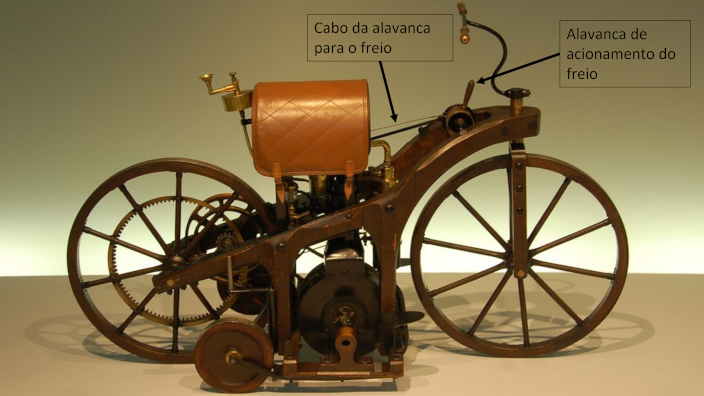
\includegraphics[width=8cm]{figuras/primeira-motocicleta-0.5cv-velocidade-maxima-12kmh.PNG}}
    }{
        \Fonte{\href{https://en.wikipedia.org/wiki/Daimler_Reitwagen}{wikipedia.org}}
    }	
\end{figure}

Outra aparição um ano depois, foi na carruagem Daimler Figura~\ref{fig:Carruagem-Daimler}, com motores de combustão interna
1,1 cv e velocidade máxima de 16 km/h, o freio de sapata era instalado na frente das rodas traseiras e era acionado pisando no mesmo.

\begin{figure}[h!]
    \centering
    \Caption{\label{fig:Carruagem-Daimler} Carruagem Daimler 1886 }	
    \UNIFORfig{}{
        {\includegraphics[width=8cm]{figuras/carruagem-daimler-1886.png}}
    }{
        \Fonte{\href{https://pin.it/2lkAp6m}{Pinterest}}
    }	
\end{figure}

\subsection{Freios de banda e sapatas externas }

À medida que os pneus de borracha sólida rapidamente se estabeleceram para veículos motorizados (começando com o automóvel triangular Benz em 1886 e o carro com rodas de aço Daimler de 1889) e logo foram substituídos por pneus de borracha cheios de ar para um conforto mais confortável. passeio, a era do freio de sapata nos automóveis já havia chegado ao fim. 

A partir de então, começaram a ser utilizados freios de banda (faixas de freio de aço flexíveis que freavam diretamente ou por meio de diversas sapatas de freio rebitadas por dentro) ou freios de sapata externos (ferro fundido rígido ou sapatas de freio de aço com lonas de freio). Esses freios acionados por pedal funcionavam com tambores de freio externos que normalmente eram instalados na frente, no eixo de transmissão intermediário ou no eixo de transmissão, na área da roda traseira. Por exemplo, a Fahrzeugfabrik Eisenach produziu o primeiro automóvel Wartburg em 1898. O Modelo 1 apresentava uma transmissão exposta e pinhões de transmissão. Os freios de banda frearam tanto o eixo quanto as duas rodas traseiras. 

Em 1899, o carro com rodas de aço da Daimler tinha pneus de borracha maciça e freios de banda de aço nas rodas traseiras (Fig. 4). O Daimler “Phoenix”, também datado de 1899, ainda tinha pneus de borracha maciça, mas estes foram logo substituídos por pneus cheios de ar. Um freio de pé atuou como freio de sapata externo no eixo de transmissão dianteiro (Figuras 5 e 6), e o freio de mão atuou nas rodas traseiras. Além disso, este carro apresentava – tal como, por exemplo, o carro de corrida Benz de 1899 (Fig. 7) – um “freio sprag”, uma haste forte montada na parte traseira que tinha a finalidade de ser conduzida contra o (normalmente relativamente). estrada suave). 

Um trecho do texto original do manual do usuário do “Phaeton” de Benz \& Co. Rheinische Gasmotoren-Fabrik AG Mannheim de 1902 diz o seguinte: “Além de um freio de mão preso no lado esquerdo, o carro é freado principalmente por pressionando o pedal esquerdo, que funciona como freio de banda nos discos de freio fixados nas duas rodas traseiras. Simultaneamente, como mencionado acima, a correia é automaticamente movida para fora. Para parar o carro imediatamente, os pedais esquerdo e direito são pressionados ao mesmo tempo, o que faz com que o freio de fita conectado ao pedal direito atue sobre o disco de freio e freie a caixa de redução.”

\subsection{Freios a tambor de sapata interna com acionamento mecânico por cabo} 

Com o tempo, os veículos tornaram-se mais rápidos e pesados. Portanto, eles precisavam de um sistema de freio mais eficaz. Assim, os freios de banda e de sapata externa logo deram lugar ao freio de tambor de sapata interno, para o qual Louis Renault solicitou uma patente em 1902. Um mecanismo de espalhamento empurrava duas sapatas de freio em forma de crescente contra a superfície interna do freio de ferro fundido ou aço. tambores, que estavam conectados à roda. Devido ao seu efeito de auto-reforço, o freio a tambor apresenta forças operacionais baixas em comparação com as forças de frenagem, longos períodos de manutenção e lonas de longa duração. 

Inicialmente, a força de frenagem era transmitida aos dois freios a tambor das rodas traseiras por meio de cabos de freio. 

Por exemplo, o Mercedes Simplex já apresentava freios a tambor adicionais nas rodas traseiras operados por cabo (Fig. 8), além do freio de banda do eixo cardan. Devido ao maior desempenho do motor (40 cavalos de potência), foi adicionado um segundo freio de pé (Fig. 9), que também atuou como freio de faixa no eixo intermediário da transmissão por corrente. A propósito, todos os quatro freios eram resfriados por um jato de água que, durante a frenagem, pingava de um reservatório nas superfícies de atrito. 

A partir de cerca de 1920, os veículos foram equipados com freios a tambor nas quatro rodas. A força de frenagem ainda era transmitida por meios mecânicos, ou seja, alavancas, juntas e cabos de freio.
    
Esses freios a tambor operados por cabo permaneceram em uso por muito tempo. Um exemplo foi o modelo padrão da VW da década de 1950 (Fig. 10): 

O elemento principal deste sistema de freio era um trilho de pressão do freio (Item 1). Os quatro cabos de freio (2) fixados a este elemento corriam para trás através das mangas dos cabos até os freios das rodas (freios a tambor) das quatro rodas (3). A parte traseira do trilho era sustentada por uma alavanca curta que ficava no eixo do pedal do freio. Quando o pedal do freio (4) foi pressionado, o trilho de pressão do freio foi empurrado para frente com os quatro cabos. Os cabos transmitiram a força aos freios das rodas. 

A alavanca do freio de mão (5) ficava mais atrás no carro. Contudo, por meio de uma haste desacoplada, o freio de mão atuava, em última análise, sobre o mesmo mecanismo que o freio de pé e, portanto, atuava igualmente sobre as quatro rodas.
    
\subsection{Acionamento do freio hidráulico }

O principal problema do freio a cabo era o grande esforço de manutenção e o efeito de frenagem desigual causado pelo atrito desigual durante a transmissão mecânica. 

Isso foi remediado quando a Lockheed introduziu um freio acionado hidraulicamente em 1919. Um fluido de freio especial agora transmitia a força do pedal do freio uniformemente aos cilindros de atuação dos freios das rodas mediante linhas e mangueiras de metal, sem a necessidade de alavancas, juntas e freios. cabos. 

A ativação do freio hidráulico também possibilitou amplificar a pressão do pé aplicada pelo motorista usando a depressão do coletor de admissão como fonte de energia para um sistema servo de freio. O princípio foi patenteado em 1919 pela Hispano-Suiza. 

Em veículos comerciais e material circulante ferroviário, os freios pneumáticos estabeleceram-se como o sistema de escolha.

Em 1926, o “Adler Standard” foi o primeiro automóvel na Europa a ser equipado com um sistema de travagem hidráulico. O primeiro reforço hidráulico da força de travagem nas corridas de automóveis foi utilizado no Mercedes-Benz “Silver Arrows” em 1954. Este acabou por se tornar equipamento padrão para muitos veículos de produção em massa. 

Como uma possível falha do circuito de freio poderia desabilitar completamente os primeiros freios de circuito único, o freio de circuito duplo foi posteriormente prescrito por lei. Conforme o desenvolvedor do VW Golf, Dr. Ernst Fiala, os primeiros “Beetles” (o modelo padrão dos VWs) ainda tinham um freio acionado por cabo exatamente por esse motivo: na época, temia-se que uma mangueira nos freios hidráulicos pudesse explodir. Mais tarde, porém – mesmo que apenas por razões competitivas – o \textit{VW Export} e o \textit{VW Transporter} apresentavam sistemas de travagem hidráulicos.

\subsection{Freio a disco }

Embora a montadora britânica Lancaster tenha patenteado o freio a disco em 1902, demorou muito até que esse tipo de freio fosse introduzido. Só cerca de cinquenta anos mais tarde, a partir de 1955, é que o lendário Citroën DS-19 se tornou o primeiro automóvel produzido em massa a ser equipado com freios de disco. O freio a disco foi derivado do freio multi-disco e foi desenvolvido inicialmente para a indústria aeronáutica. 

No freio a disco, uma lona de freio pressiona o disco de freio por dentro e por fora. O disco de freio (normalmente feito de ferro fundido ou, menos comumente, de aço) é conectado à roda. Sua vantagem é a estrutura simples e de fácil montagem. Também neutraliza a redução do efeito de travagem causado pelo sobreaquecimento e evita o desalinhamento das rodas de um eixo. 

O primeiro carro alemão com freios a disco nas rodas dianteiras foi o BMW 502 em 1959. Os primeiros carros alemães a ter freios a disco nas quatro rodas foram o Mercedes 300 SE, o Lancia Flavia e o Fiat 2300 em 1961. Hoje, praticamente todos os carros possuem sistema de freio a disco, pelo menos nas rodas dianteiras. Em 1974, foram introduzidos os primeiros carros de corrida de Fórmula 1 com discos de freio compostos de fibra de carbono. Esses discos são considerados especialmente leves e resistentes ao calor e, portanto, ganharam amplo uso no automobilismo e na aviação.

\subsection{Pastilhas e sapatas de freio} 

Foi necessário desenvolver lonas de freio adequadas para freios a tambor e a disco, para os quais o amianto provou ser particularmente eficaz. Só quando se soube que as fibras de amianto eram prejudiciais à saúde é que o material foi substituído pela fibra plástica.

\subsection{Sistemas de estabilidade de condução }

A era dos sistemas de travagem eletrônicos começou em 1978 com a chegada do sistema de travagem anti bloqueio (ABS) para automóveis desenvolvidos pela Bosch. Durante a frenagem, o ABS fornece detecção precoce do travamento incipiente de uma ou mais rodas e evita o travamento das rodas. Garante a dirigibilidade do veículo e reduz substancialmente o perigo de derrapagem. Em 1986, foi seguido pelo sistema de controlo de tração (TCS), com o qual a Bosch alargou a capacidade do sistema para o controlo da patinagem das rodas sob aceleração. A Fig. 11 mostra testes de estrada destes sistemas no campo de testes da Bosch em Boxberg, no sul da Alemanha.

Como uma melhoria adicional na segurança de condução, a Bosch introduziu o programa eletrônico de estabilidade (ESP) em 1995, que integra as funções do ABS e do TCS. Ele não apenas evita que as rodas do veículo travem e girem, mas também evita que o veículo puxe para o lado. Sistemas alternativos, como a direção nas quatro rodas e a cinemática do eixo traseiro, desenvolvidos nas décadas de 1980 e 1990 e foram instalados em alguns veículos de produção em massa, não se popularizaram porque pesavam muito e custavam muito caro. ou não foram suficientemente eficazes.

Enquanto isso, o controle de freio \textit{sen sotronic} (eletro-hidráulico) encontrou seu lugar na construção de automóveis. Fornece todas as funções do ESP e desacopla o funcionamento mecânico do pedal do freio por meio de um sistema de controlo eletrônico. Por motivos de segurança, um sistema hidráulico de reserva está automaticamente disponível.

\section{Classificação dos sistemas de travagem dos automóveis}

Todos os sistemas de frenagem de um veículo são chamados de equipamentos de frenagem. Os sistemas de freio dos automóveis podem ser classificados com base em

\begin{itemize}
    \item design e
    \item método de operação
\end{itemize}

\subsection{Designs}

Com base nos requisitos legais, as funções do equipamento de travagem são partilhadas entre três sistemas de travagem:

\begin{itemize}
    \item os freios de serviço,
    \item o sistema de freio secundário, e
    \item o freio de estacionamento
\end{itemize}

Nos veículos comerciais, o equipamento de travagem também inclui um sistema de travagem de funcionamento contínuo (por exemplo, retardador) que permite ao condutor manter o veículo a uma velocidade constante numa descida longa. O equipamento de travagem de um veículo comercial inclui também um sistema de travagem automático que acciona os freios de um reboque se este for desengatado do veículo trator, deliberadamente ou por acidente.

\subsection{Freios de serviço}

O sistema de freio de serviço (“freio de pé”) é utilizado para desacelerar o veículo, manter sua velocidade constante em uma descida ou pará-lo completamente. 

O condutor pode variar infinitamente o efeito de travagem através da pressão aplicada no pedal do travão. O sistema de freio de serviço aciona os freios nas quatro rodas.

\subsection{Sistema de freio secundário }

O sistema de freio secundário deve ser capaz de fornecer pelo menos algum grau de frenagem caso o sistema de freio de serviço falhe. Deve ser possível variar infinitamente o nível de travagem aplicado. 

O sistema de freio secundário não precisa ser um terceiro sistema de freio totalmente separado (além dos freios de serviço e do freio de estacionamento) com seu próprio dispositivo de atuação separado. Pode consistir no circuito intacto restante de um sistema de freio de serviço de circuito duplo no qual um circuito falhou, ou pode ser um freio de estacionamento capaz de aplicação gradual.


\subsection{Sistema de freio de estacionamento }

O freio de estacionamento (freio de mão) desempenha a terceira função exigida do equipamento de freio. Deve impedir que o veículo se mova quando parado ou estacionado, mesmo em declive e quando o veículo estiver desacompanhado. 

Conforme os requisitos legais, o sistema de freio de estacionamento também deve ter uma ligação mecânica intacta, por ex. uma ligação de haste ou cabo, entre o dispositivo de atuação e os freios que ele opera. 

O sistema de freio de estacionamento é geralmente accionado por meio de uma alavanca do freio de mão posicionada perto do banco do condutor ou, em alguns casos, por um pedal. Isto significa que os sistemas de freio de serviço e de estacionamento de um veículo motorizado possuem dispositivos de atuação e meios de transmissão de força separados. 

O sistema de freio de estacionamento é capaz de aplicação gradual e aciona os freios apenas em um par de rodas (dianteiras ou traseiras)


\section{Métodos de operação}

Dependendo de serem operados total ou parcialmente pelo esforço humano, ou por outra fonte de energia, os sistemas de travagem podem ser classificados como

\begin{itemize}
    \item sistemas de frenagem de energia muscular (não assistida),
    \item sistemas de travagem assistidos, ou
    \item sistemas de freio elétrico,
\end{itemize}

\subsection{Sistemas de frenagem de energia muscular }

Neste tipo de sistema de frenagem, frequentemente encontrado em carros e motocicletas, o esforço aplicado ao pedal do freio ou à alavanca do freio de mão é transmitido aos freios de forma mecânica (por meio de uma haste ou cabo) ou hidraulicamente. A energia pela qual a força de travagem é gerada é produzida inteiramente pela força física do condutor.

\subsection{Sistemas de travagem assistida }

O sistema de travagem assistida é o tipo mais comumente utilizado em automóveis e veículos comerciais ligeiros. Amplifica a força aplicada pelo motorista por meio de um servofreio que utiliza outra fonte de energia (vácuo ou hidráulica). A potência muscular amplificada é transmitida hidraulicamente aos freios.

\subsection{Sistemas de freios elétricos }

Os sistemas de freios elétricos são geralmente usados em veículos comerciais, mas são ocasionalmente instalados em carros grandes em conjunto com um sistema ABS integral. Este tipo de sistema de travagem é operado inteiramente sem energia muscular.

O sistema é operado por energia hidráulica (que se baseia na pressão do fluido) transmitida por meios hidráulicos. O fluido de freio é armazenado em acumuladores de energia (acumuladores hidráulicos) que também contêm um gás comprimido (geralmente nitrogênio). O gás e o fluido são mantidos separados por um diafragma flexível (acumulador de diafragma) ou um pistão com vedação de borracha (acumulador de pistão). Uma bomba hidráulica gera a pressão do fluido, que está sempre em equilíbrio com a pressão do gás no acumulador de energia. Um regulador de pressão coloca a bomba hidráulica em marcha lenta assim que a pressão máxima é atingida.

Como o fluido de freio pode ser considerado praticamente incompressível, pequenos volumes de fluido de freio podem transmitir grandes pressões ao sistema de freio.


